Figure \ref{fig:softwareArchitecture} shows a high-level overview of the 
software architecture. The Benchmarking system is based on a message bus 
architecture. The figure further shows the core architectural components of
the system.

\begin{figure}[H]
  \begin{center}
  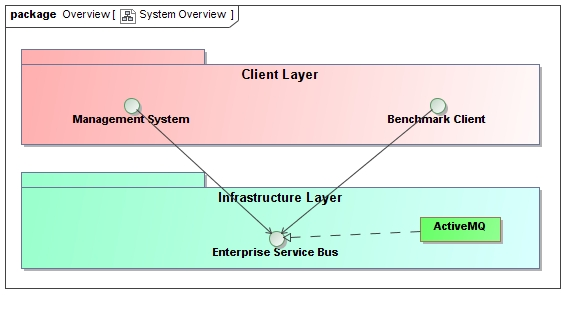
\includegraphics[scale=0.4]{../Diagrams and Charts/Overview/SystemOverview.jpg}
  \caption{A high-level overview of the software architecture for the Benchmarking Service}
  \label{fig:softwareArchitecture}
  \end{center}
\end{figure}

\section{Management System}
Figure \ref{fig:managementSoftwareArchitecture} shows a high-level overview of
the management service software architecture. The management service is based
on a layered architecture. The figure further shows the core architectural
components of the subsystem.

\begin{figure}[H]
  \begin{center}
  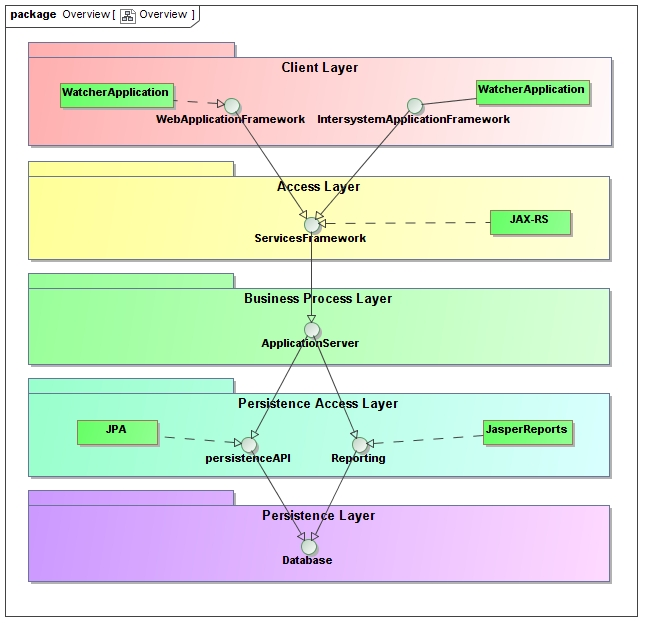
\includegraphics[scale=0.4]{../Diagrams and Charts/Overview/Overview.jpg}
  \caption{A high-level overview of the software architecture for the Management Service}
  \label{fig:managementSoftwareArchitecture}
  \end{center}
\end{figure}

\section{Benchmark Client}
